% \vspace*{-1.2cm}
\section{Συμπεράσματα \& παρατηρήσεις}

\begin{table}[H]
	\begin{center}
		\begin{tabular}{|c|c|}
			\hline
			\multicolumn{2}{|c|}{\textbf{Aspect ratios}}                                \\\hline
			$S_1 = 70$                   & $S_5 = 30$                                   \\\hline
			$S_2 = 70$                   & $S_6 = 20$                                   \\\hline
			$S_3 = 30$                   & $S_7 = 40$                                   \\\hline
			$S_4 = 30$                   & $S_8 = 6$                                    \\\hline\hline
			\textbf{Χωρητικότητα Miller} & $C_C=0.477 \unit{\pico\farad}$               \\\hline
			\textbf{Αντίσταση μηδενικού} & $R_Z=500\kohm$                               \\\hline
			\textbf{Ρεύμα αναφοράς}      & $I_{\mathrm{ref}} = 20\unit{\micro\ampere}$ \\\hline
		\end{tabular}
		\label{table:final_params}
		\caption{Παράμετροι του κυκλώματος \ref{circ:op_amp_sim}. Τα μήκη των διαύλων όλων των transistor είναι $L=1\unit{\micro\meter}$}
	\end{center}
\end{table}

\begin{table}[H]
	\begin{center}
		\begin{tabular}{|r|l|}
			\hline
			\textbf{Κέρδος ανοιχτού βρόχου} & $20\cdot\log_{10}{\(A_v\)}=25.55619\unit{\decibel}$   \\\hline
			\textbf{Gain-bandwidth product} & $\mathrm{GB}=8.70313\unit{\mega\hertz}$               \\\hline
			\textbf{Περιθώριο φάσης}        & $\phi_M=59.95727^\circ$                               \\\hline
			\textbf{Κατανάλωση ισχύος}      & $P_{\mathrm{diss}}=0.928\unit{\milli\watt}$        \\\hline
			\textbf{Slew rate}              & $\mathrm{SR}=69.20035\:\unit{\volt\per{\micro\second}}$ \\\hline
		\end{tabular}
		\label{table:final_specs}
		\caption{Αποτελέσματα προσομοιώσεων του κυκλώματος \ref{circ:op_amp_sim}.}
	\end{center}
\end{table}

Αποσυνδέοντας το δίκτυο ανάδρασης, και γειώνοντας και τις δύο εισόδους του τελεστικού ενισχυτή παρατηρήθηκε μη μηδενική έξοδος (διάγραμμα \ref{plot:offset}), παρόλο που έχει ακολουθηθεί η σχετική οδηγία, \eqref{eq:S7a}, περί τάσης εκτροπής. Προφανώς, η αποφυγή του συστηματικού dc offset σε μία πρακτική εφαρμογή είναι πιο περίπλοκη. Ωστόσο, να σημειωθεί πως τα ζεύγη M1-M2 και M3-M4 είναι μεταξύ τους πανομοιότυπα και το ρεύμα των drain ακροδεκτών τους είναι ίδιο και για τα τέσσερα.\par
Αρχιτεκτονικές πιο σύνθετες από αυτήν των δύο σταδίων και διαφορετικές τεχνολογίες κατασκευής MOSFET θα μπορούσαν να παρέχουν ακόμη μεγαλύτερο κέρδος τάσης και gain-bandwidth ή και υψηλότερο slew rate. Θα μπορούσαν επίσης να βελτιώσουν το θερμοκρασιακό εύρος λειτουργίας του ενισχυτή.\par

\begin{center}
	\begin{plotenv}[H]
		\centering
		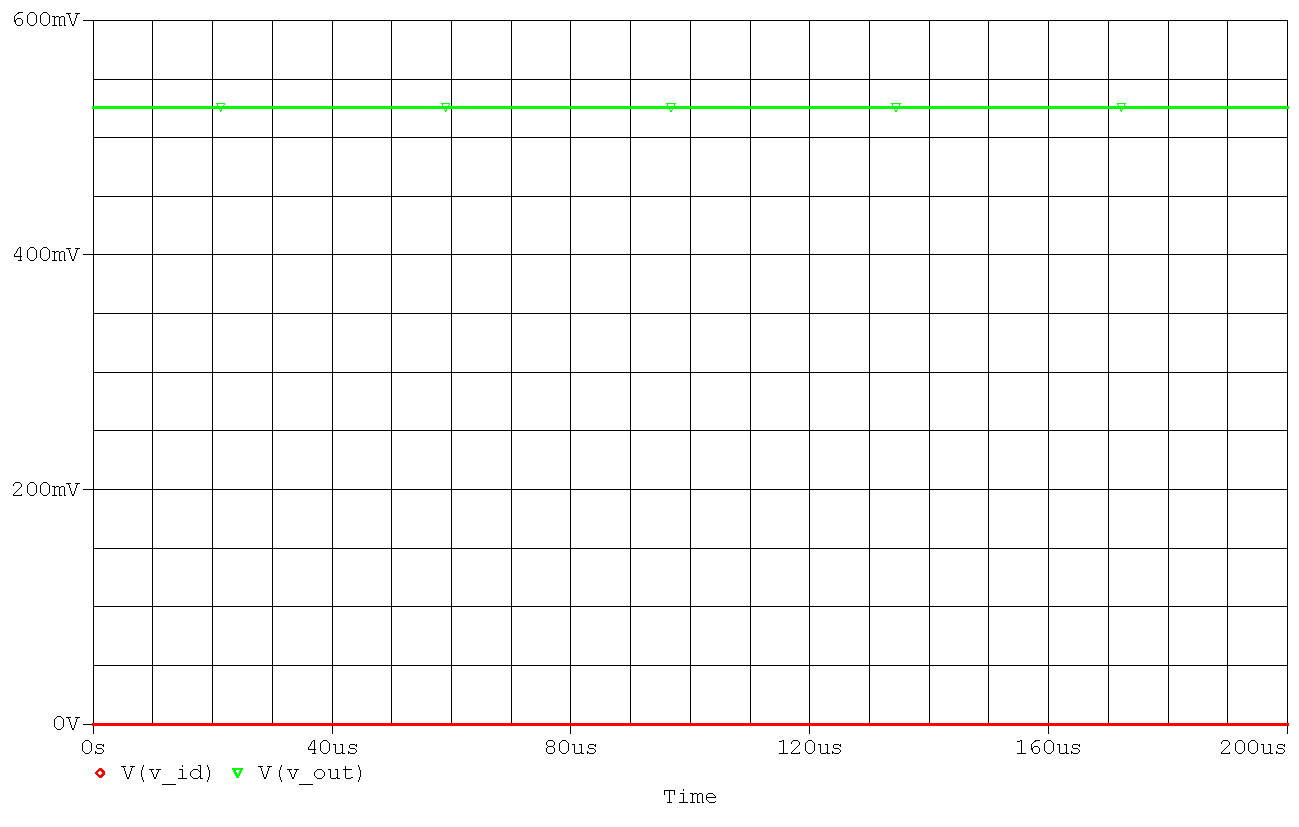
\includegraphics[width=\linewidth]{op_amp_sim/dc_offset.pdf}
		\caption{Με κόκκινο χρώμα διαγράφεται η διαφορική είσοδος και με πράσινο χρώμα η έξοδος του τελεστικού ενισχυτή. Το δικτύωμα ανάδρασης έχει αποσυνδεθεί και οι είσοδοι του ενισχυτή είναι βραχυκυκλωμένες στη γείωση. Η έξοδος είναι $v_{\mathrm{out}}=525.59128\unit{\milli\volt}$}
		\label{plot:offset}
	\end{plotenv}
\end{center}